% !TeX program = xelatex
\documentclass{tudelft-report} %[whitelogo]
\usepackage{algorithm}
\usepackage{algpseudocode}
\usepackage{amsmath}
\usepackage{blindtext}	% TODO Remove
\usepackage{changes}
\usepackage[nameinlink,capitalise]{cleveref}
\usepackage{enumitem}
\usepackage{amsbsy}
\usepackage{afterpage}
\usepackage{hyperref}
\usepackage[acronym]{glossaries} % toc does not work properly
\usepackage{siunitx}
\usepackage{subcaption} 
\usepackage{tikz}

\usetikzlibrary{automata,arrows,shapes}

\makeglossaries

\graphicspath{{./figures/}}

%% Glossary and Acronyms %%
%% List of acronyms %%
% Reference definition:
% - \newacronym[options]{label}{short}{long}
%	options: description, longplural, ...
%
% Reference usage:
% - \acrlong{label}  : displays the full text of the acronym
% - \acrshort{label} : displays the abbreviation
% - \acrfull{label}  : displays the full text followed by the abbreviation
% - \acrshortpl{label} : the plural of the abbreviation (similarly for acrlongpl and acrfullpl)

\newacronym{acr:dtp}{DTP}{Decision-Theoretic Planning}

\newacronym{acr:hmm}{HMM}{Hidden Markov Model}

\newacronym[longplural=Markov Decision Processes]{acr:mdp}{MDP}{Markov Decision Process}

\newacronym{acr:pomdp}{POMDP}{Partially Observable \acrshort{acr:mdp}}

\newacronym{acr:sdm}{SDM}{Sequential Decision Making}
%% Glossary Entries:
%
% Reference definition:
% \newglossaryentry{maths}
% {
% 	name=mathematics,
% 	description={Mathematics is what mathematicians do}
% }
%
% Reference usage:
% - \gls{ } Prints term lower case
% - \Gls{ } Prints term upper case
% - \glspl{ } Prints term plural lower case
% - \Glspl{ } Prints term plural upper case

\newglossaryentry{maths}{
	name={mathematics},
	description={Mathematics}
}

\newcommand\mat[1]{\pmb{#1}}
\newcommand\arr[1]{\pmb{#1}}
\DeclareMathOperator*{\argmax}{arg\,max}

%% Custom Definitions %%
\def\subsubsectionautorefname{Section}
\def\subsectionautorefname{Section}
\def\sectionautorefname{Section}
\def\chapterautorefname{Chapter}
\def\algorithmautorefname{Algorithm}

%% Pseudocode settings %%
\newcommand*\Let[2]{\State #1 $\gets$ #2}
\algrenewcommand{\algorithmiccomment}[1]{\hfill$\rhd$ #1} % Fix for comments in pseudocode

%% Title and Cover Pages %%

%% Use Roman numerals for the page numbers of the title pages and table of
%% contents.
\frontmatter

%% Uncomment following 16 lines for a cover with a picture on the lower half only
\title[tudelft-white]{Learning and Optimizing Probabilistic Models for Planning Under Uncertainty in Mobile Robot Navigation}
%\subtitle[tudelft-black]{Optional subtitle}
\author[tudelft-white]{R. van Bekkum}
\affiliation{Delft University of Technology}
\coverimage{figures/tank.jpg}
\covertext[tudelft-white]{
	\textbf{Cover Text} \\
	possibly \\
	spanning 
	multiple 
	lines
	\vfill
	ISBN 000-00-0000-000-0
}
\setpagecolor{tudelft-cyan}
%\makecover[split]

% TEMPORARY
\newcommand{\showoutline}[1]{
	\vspace{0.3cm}
	\hrule
	\vspace{0.3cm}
	{\large\textbf{PLANNED OUTLINE}:}
	\vspace{0.3cm}
	\hrule
	\vspace{0.3cm}
	{#1}
	\vspace{0.3cm}
	\hrule
	\vspace{0.3cm}	
}

\begin{document}

%% Include an optional title page.
\begin{titlepage}


\begin{center}

%% Insert the TU Delft logo at the bottom of the page.

%% Print the title in cyan.
{\makeatletter
\largetitlestyle\fontsize{36}{94}\selectfont\@title										% TODO Change font size here
%\largetitlestyle\color{tudelft-cyan}\Huge\@title
\makeatother}

%% Print the optional subtitle in black.
{\makeatletter
\ifx\@subtitle\undefined\else
    \bigskip
   {\tudsffamily\fontsize{22}{32}\selectfont\@subtitle}    
    %\titlefont\titleshape\LARGE\@subtitle
\fi
\makeatother}

\bigskip
\bigskip

by
%door

\bigskip
\bigskip

%% Print the name of the author.
{\makeatletter
%\largetitlefont\Large\bfseries\@author
\largetitlestyle\fontsize{20}{26}\selectfont\@author
\makeatother}

\bigskip
\bigskip

to obtain the degree of Master of Science

at the Delft University of Technology,

to be defended publicly on Tuesday July xx, 2017 at 10:00 AM.

\vfill

\begin{tabular}{lll}
    Student number: & 4210816 \\
    Project duration: & \multicolumn{2}{l}{November 14, 2016 -- July xx, 2017} \\
    Thesis committee: & Dr.\ M.\ T.\ J.\ Spaan, & TU Delft, supervisor \\
        & Dr.\ P.\ Pietersen, & TU Delft \\												% TODO Update
        & Ir.\ A.\ Aaronson, & Acme Corporation											% TODO Update
\end{tabular}
%% Only include the following lines if confidentiality is applicable.

\bigskip
\bigskip
\emph{This thesis is confidential and cannot be made public until July xx, 2017.}
%\emph{Op dit verslag is geheimhouding van toepassing tot en met 31 december 2013.}

\bigskip
\bigskip
An electronic version of this thesis is available at \url{http://repository.tudelft.nl/}.
%\\[1cm]

%\centering{\includegraphics{cover/logo_black}}


\end{center}

\begin{tikzpicture}[remember picture, overlay]
    \node at (current page.south)[anchor=south,inner sep=0pt]{
        \includegraphics{cover/logo_black}
    };
\end{tikzpicture}

\end{titlepage}



\chapter*{Abstract}
\label{ch:abstract}

Motion and path planning in robotics are some of the many applications that require agents that account for uncertainty in the form of action failures or disturbances caused by exogenous events.
A typical approach for planning in these domains involving uncertainty is to set up a probabilistic model of the environment, a typical choice being a Markov Decision Process (MDP), and apply existing decision-theoretic planning techniques to obtain an optimal plan.
However, devising these probabilistic models usually requires expert knowledge on the domain and might be a daunting and error-prone task.
Therefore it is desirable to automate the process of obtaining probabilistic models through learning algorithms.
Even though some work has already been done on crafting such learning algorithms, most of these algorithms assume the state-space of the model to be already known.
In this work we propose a method that autonomously learns MDPs solely from execution traces obtained from an exploration phase.
From these execution traces the state spaces of MDPs are learned by applying unsupervised machine learning methods.
The model quality is assessed by running simulations of the system using policies from standard MDP solvers, and in order to obtain the best MDP model, Bayesian Optimization is applied over the parameter space of the machine learning method.
The approach is tested for mobile robot navigation, as the robots in this domain oft to operate under significant uncertainty in their actions.

%
%\vspace{12pt}
%\noindent\fbox{\textbf{TODO:} Needs to be slightly updated.}
%

%The approach is tested for mobile robot navigation, as the robots in this domain operate under significantly uncertainty and can illustrate the method well as positions can be mapped to states and actions are limited to a finite set of rotations and translations.

\chapter*{Preface}
\setheader{Preface}

%
\vspace{12pt}
\noindent\fbox{\textbf{TODO:} Preface chapter needs to be written.}
%

\begin{flushright}
{\makeatletter\itshape
    \@author \\
    Delft, July 2017
\makeatother}
\end{flushright}



\tableofcontents

\listoffigures

%\listofalgorithms

%% Use Arabic numerals for the page numbers of the chapters.
\mainmatter

\chapter{Introduction}
\label{ch:introduction}

In numerous real-world settings, such as traffic light control \cite{wiering2004intelligent}, mobile robot navigation \cite{MartinezCantin2009} or decision-making in medical treatment \cite{schaefer2005modeling}, it is quite common to be faced with uncertainty about the effect of an action (possibly selected based on incomplete or faulty observations).
Therefore, when plans are provided to impose a course of action for such settings, they need to be more sophisticated, anticipating for the observations that might be made and being able to act accordingly.
That is, a proper trade-off should be made between the different possible outcomes and the costs of executing a plan.

A general approach for \textit{planning under uncertainty} is to model the dynamics of the system in need of automated control, defining transition probabilities for moving between attainable states through the selection of actions.
Typically such models are handcrafted by a human designer, although this is often a daunting and time-costly process.
Therefore, an appealing alternative is to employ learning algorithms to obtain these models from a dataset describing the dynamics of the system.
The state of the art does however lack a method of properly tuning the hyper-parameters of these learning algorithms so to maximize the performance yielded by executing the plans derived from learned models.
To address this problem, this thesis proposes a framework that effectively optimizes for a performance-maximizing model for a system in need of automated control.

\section{Motivation}
\label{sec:motivation}

There exist several practical applications in which the (sequential) actions of systems are coordinated by decision makers or \textit{agents} to achieve long-term goals.
In particular these agents need to take into account the uncertainty in these systems that may be present in the form of action failures, exogenous events and noisy observations.
%An example application in which the system faces such uncertainty is that of mobile robot navigation, in which the system is in need of automated control taking into account the possibility of the robot slipping, running into obstacles and producing noisy sensor readings.
To devise optimal plans for those systems whose dynamics are stochastic, \acrfull{acr:dtp} aims to account for uncertainty by exploiting the considerable structure these systems pose through the development of probabilistic models which reflect this uncertainty.
These probabilistic models serve as a system representation which describe a system's state and its evolution over time after a sequence of actions has been executed.
The advantage of having such (accurate) probabilistic models at one's disposal is that agents can act according to different policies derived from one and the same model to perform multiple tasks.

In recent years particularly \acrfullpl{acr:mdp} have become a significant popular formalism for modeling \acrshort{acr:dtp} problems \cite{Boutilier1999}. 
That is, first of all, due to their firm foundation in decision theory and successes of Markovian approaches in speech recognition \cite{baker1992large, gales2008application, rabiner1989tutorial} and the closely-related field of \acrfull{acr:rl} \cite{kaelbling1996reinforcement, Brafman2002}.
Furthermore, over the years various computationally efficient solution techniques have been devised for obtaining optimal plans for \acrshort{acr:mdp} models which maximize expected value (e.g.,  \cite{puterman2014markov, howard1960dynamic}).
Considering the expediency of \acrshortpl{acr:mdp} for automated control, it seems worthwhile to investigate methods of developing accurate probabilistic models for the purpose of planning under uncertainty.

% New paragraph here

% Mainly applied approach in automated control involves hand-crafting a mathematical model as a system representation that can be used to represent the system's state and its evolution over time after a sequence of actions has been executed.
% Setting up such models is an important, difficult and time-costly process for human designer that might not always have (enough) expertise to craft a suitable model that can be used to plan for the execution of tasks.

%\newpage

\section{Problem Statement}
\label{sec:problem-description}

\begin{figure}[t]
	\centering
	\includegraphics[width=\textwidth]{high-level-planning-diagram-cropped}
	\caption{Diagram showing a typical iterative procedure followed in the development of probabilistic models for planning under uncertainty. Given a problem description for the real-world system under consideration, a designer refines the model until satisfactory performance is observed.}
	\label{fig:high-level-model-development}
\end{figure}

The problem this thesis is concerned with is the development of probabilistic models, which are used for obtaining plans for automated control of systems whose dynamics are stochastic.
Setting up such models is an important, though difficult and time-costly process for a human designer that might not always have (enough) expertise to craft a suitable, well-generalizing model that can be used to plan for the execution of different tasks.
In practice, this problem is tackled by domain experts by iteratively tweaking the model parameters until the desired performance is achieved.
%The typical procedure is depicted in \autoref{fig:high-level-model-development} in which is seen that the model parameters are updated until satisfactory performance is observed.

\autoref{fig:high-level-model-development} shows a typical procedure followed in the design of a probabilistic model.
In this procedure, the human designer is presented a problem description and handcrafts an initial model for the system.
The model is then evaluated by performing tasks following the plans that are derived from the model in simulations or even in the real world.
The assessed performance steers the designer towards what model parameters appear to work well.
The designer uses the obtained knowledge to iteratively refine the model parameters until ultimately satisfactory performance is yielded in the execution of the derived plans.

An alternative that one ought to consider, is that of applying \acrshort{acr:rl} techniques rather than planning algorithms.
However, although ideas from planning and \acrshort{acr:rl} are interchangeable, these techniques typically demand direct interaction with the environment which is something that cannot always be readily offered.
That is, \acrshort{acr:rl} techniques turn out as time-consuming and sometimes even riskful or dangerous when applied in real-world environments.
Those domains for which plans need to be formulated offline, demand the acquisition of probabilistic models which accurately define what constitutes the state of the system, reflect uncertainty through transition probabilities and specify its goals in some manner.%TODO Rewrite 'some manner of specifying goals'?

An attractive approach of bypassing the daunting and error-prone task of handcrafting probabilistic models, is that of automatizing the model development process by applying learning algorithms on data that describes the dynamics of the system.
For this approach the data is typically presented in the form of execution traces of the system operating in a real-world environment, which is collected in an exploration phase prior to the actual planning.
However, although one could obtain a model of the system by applying learning algorithms, the corresponding plans that are inferred from this model might not be effective when applied in a real-world environment.
First of all, this might be due to the parameters of the learning algorithm not being set properly, signifying the need for proper adjustment of these parameters.
Another possibility is that the gathered data is incomplete and so does not accurately describe the dynamics of the system.
In this case, one could choose to augment the data for those areas for which the training data is inadequate, although one should be aware that this is accompanied by a more cost-expensive model-learning process.
Therefore, in order to learn accurate probabilistic models, we are in need of a way of assessing the performance of a model accompanied by a method for identifying inadequacies due to incomplete data, while taking into account the corresponding cost of learning and evaluating these system models.

\section{Research Questions}
\label{sec:research-questions}
The problem statement as presented in the previous section yields the following main research question for this thesis:

\vspace{12pt}
\noindent%\fbox{\parbox{\textwidth}{ %Uncomment this for boxes
\textbf{Main Research Question.} How can the task of obtaining a \acrfull{acr:mdp} that maximizes the yielded performance of executing plans that are derived from it, given a dataset about the system under consideration, be automated?
%}}
\vspace{12pt}

To answer this main research question, four research questions have been identified which are presented below.
The relevance of each of these research questions is discussed accordingly in the next paragraphs.

\vspace{16pt}
\noindent%\fbox{\parbox{\textwidth}{
\textbf{Research Question 1.} Which learning algorithms exist that can be employed for learning \acrshortpl{acr:mdp} from data for systems involving uncertainty that require plans for automated control?
%}}
\vspace{0pt}

First off, to facilitate the formulation of plans for a system involving uncertainty, we need to obtain an \acrshort{acr:mdp} from the provided dataset.
Therefore, we should know what learning algorithms exist that can be employed to learn the parameters of an \acrshort{acr:mdp}.
Accordingly, we should identify the applications for which each of these algorithms are suited, but also what the shortcomings or vulnerabilities of each of these algorithms are.

\vspace{16pt}
\noindent%\fbox{\parbox{\textwidth}{
\textbf{Research Question 2.} How should a performance measure be defined which can be used to fairly compare the value of different \acrshortpl{acr:mdp}?
%}}
\vspace{12pt}

As various \acrshortpl{acr:mdp} can be obtained for different parameter settings of the model learning algorithms, the need for a measure of performance for different \acrshortpl{acr:mdp} emerges.
That is, to establish which parameter settings yield an \acrshort{acr:mdp} that best reflects the underlying system for the tasks to be executed, we require a way to express and fairly compare the value of the learned \acrshortpl{acr:mdp}.

\vspace{16pt}
\noindent%\fbox{\parbox{\textwidth}{
\textbf{Research Question 3.} How can the parameter space of model learning algorithms cost-effectively be explored towards a global maximizer with only limited knowledge about the system under consideration?
%}}
\vspace{12pt}

A model learning algorithm may yield different \acrshortpl{acr:mdp} depending on the selected parameter settings.
To establish the most appropriate \acrshort{acr:mdp} for the system under consideration, the performance yielded by multiple \acrshortpl{acr:mdp} should be compared.
As evaluating all possible parameter-settings would be cost-expensive, we need to investigate other ways of exploring the parameter space more cost-effectively.
This is under the assumption that we only have limited to no belief over which parameter-settings might work well for the system under consideration.

\vspace{16pt}
\noindent%\fbox{\parbox{\textwidth}{
\textbf{Research Question 4.} How can the hierarchy of different abstraction levels be exploited to find a performance-maximizing \acrshort{acr:mdp} in a more cost-effective way?
%}}
\vspace{12pt}

Assessments of performance can be made at different levels of abstraction of the underlying system.
That is, we could examine how well an agent would perform a task only from the perspective of the \acrshort{acr:mdp} model, but also
from simulations or even the real world.
At the one hand abstracting from the real world typically yields a less accurate representation of the reality, although on the other hand assessing the performance from a more abstract level is accompanied by smaller computational costs.
Therefore, it might be valuable to investigate how this could be exploited to achieve a more cost-effective optimization of the performance.

%\vspace{12pt}
%\noindent\textbf{Research Questions:}
%\begin{enumerate}[label=\textbf{\arabic*})]
%	\item Which methods exist for learning (probabilistic) models from data for a system involving uncertainty that requires plans for automated control?
%	\item How should a performance measure be defined that can be used to fairly compare the value of different \acrshortpl{acr:mdp}?
%	\item How can the hierarchy of different abstraction levels be exploited to find a performance-maximizing \acrshort{acr:mdp} in a more cost-effective way?
%\end{enumerate}

\section{Contributions}
\label{sec:contribution}

We propose a framework for automating the development of probabilistic models in the form of \acrshortpl{acr:mdp} by applying learning algorithms on data describing the dynamics of the system under consideration.
The data about the environment that is used by these learning algorithms is gathered prior to the model learning process in an exploration phase.
%In order to obtain accurate probabilistic models for the system under consideration, the hyper-parameters of the used learning algorithm should be tweaked in such way to optimize the performance in the execution of its tasks.
Although various algorithms for learning \acrshortpl{acr:mdp} offline from a dataset \cite{shatkay1997learning, welch2003hidden, nikovski2002state} do already exist, the state of the art lacks a method for setting the hyper-parameters of these algorithms so to best reflect the underlying system and maximize the performance in the execution of its tasks.

%In order to obtain accurate probabilistic models for the system under consideration, the parameter-settings of the used model learning algorithm are iteratively tweaked towards a setting that maximizes the performance in the execution of the tasks expected to be performed.
%To achieve this we pose the adjustment of the learning algorithm parameters as an optimization task to maximize the performance that follows from executing plans derived from learned \acrshortpl{acr:mdp}.
To address this problem, the proposed framework poses the adjustment of the learning algorithm parameters as an optimization task of maximizing the performance that follows from executing plans derived from learned \acrshortpl{acr:mdp}.
The optimization is performed by applying a technique known as \acrfull{acr:bo}, such that we define a probability distribution over functions to model the performance measure and iteratively sample parameter-settings towards a global maximizer of the performance.
Although algorithms that employ the same framework for optimizing the parameters of probabilistic models \cite{ghavamzadeh2015bayesian, guez2012efficient} or policy search \cite{deisenroth2011pilco, wilson2014using} do exist, these are online approaches that do not utilise the available data prior to interacting with the real world environment.

%To address model inadequacies that are due to incomplete data, we propose to incorporate the identification of insufficient exploration for the transitions from those states that are visited in the execution of obtained plans.
%That is, for those learned models for which the data was observed to be incomplete, the observations of the performance for the corresponding parameter-settings are modeled as noisy or uncertain.
%This serves the purpose of more cautious exploitation of those areas of the parameter space which mostly produce noisy observations of the performance measure.

To achieve a more cost-effective optimization, the parameter search space is first narrowed down by a pre-processing step.
In this step assessments of the model value are made on a more abstract level (i.e., based on the computed value function for an \acrshort{acr:mdp}).
The posterior that follows from this step is then used to steer the acquisition in the main optimization step.

In attempt to further improve the learned models, a post-processing step is performed that aims to identify and fix discrepancies between the model and the real-world.
This post-processing step increases the resolution for those areas of the state-space when it identifies the outcomes of actions in simulations do not match the learned transition probabilities.

The framework is applied, tested and evaluated for the domain of mobile robot navigation, as the robots in this domain tend to operate under significant uncertainty in their actions.
A solution in this context is a policy which maps discretized robot poses into fine-grained navigation actions so to move a mobile robot to a certain goal location.
Probabilistic models are acquired by applying unsupervised machine learning algorithms on execution traces (consisting of odometry data describing robot poses) obtained in an exploration phase.
The optimization of the model is based on the performance of acquired models in simulations, which is expressed in terms of the time that has passed to reach multiple goal locations.
%Incomplete exploration data is here identified by inspecting the trajectories that are obtained from the execution of an optimal plan for an \acrshort{acr:mdp}.

% labeled as noisy uncertain observation of the performance of the model

% Discuss the learning and optimization routine: Automized method for learning probabilistic models in the form of MDPs by applying (machine) learning algorithms on exploration data. Optimization of the model by Bayesian Optimization based on performance in simulations.
% Identify incomplete exploration data about the environment by inspecting the observed trajectories and provide feedback on this from the optimization loop.
% Application to mobile robot navigation; A solution in this context is a policy that maps discretized robot poses into fine-grained navigation actions.

\section{Scope and Limitations}
\label{sec:scope-limitations}

First of all, we restrict ourselves to learning fully observable \acrshortpl{acr:mdp} from data.
However, this framework could possibly be extended to deal with applications where the states cannot be directly observed and should be inferred from observations.

Secondly, we note that all experiments and corresponding results are based on data that is solely obtained from simulations of a mobile robot.
Reasons for this are that we make the assumption that the environment is fully observable, which is typically not the case for real-world applications.
Another motivation of this is that the framework is not solely intended for the domain of mobile robot navigation and data from simulations is therefore deemed adequate for our experiments. % and not having a real robot at hand, which would be too expensive and comes with its own technical challenges that are outside of our scope.

Finally, we focus on the domain of mobile robot navigation to evaluate and test our approach.
One of the important aspects to consider, is which data should be collected to describe the dynamics of the system to learn models from this data.
For our implementation we choose to collect data about the robot's poses from internal odometry, but for other applications we might not be able to describe the states and transitions of the system through a geometric model and may need other learning algorithms than the clustering algorithms we use for our application.
An example of such applications might be that of learning \acrshortpl{acr:mdp} for traffic light control \cite{wiering2004intelligent, delgado2011efficient}, in which, for instance, lane-turn probabilities could be learned from a data-set.
Note that this application seems particularly appropriate to be approached in combination with \acrshort{acr:rl} techniques, so that the system is able to adapt to changes that occur over time.

% POMDPs: Restricted to MDPs, but could possible be extended to deal where the states are cannot be directly observed and should be inferred from observations.
% Field of application: We will discuss how the proposed method could be applied to other domains, although we will focus on the domain of mobile robot navigation to evaluate and test our method.

\section{Outline}
\label{sec:introduction-outline}

In this chapter we presented our motivations and defined the problem this thesis is concerned with.
To approach this problem we propose a framework that is aimed at automating the development of probabilistic models for the purpose of automated control by agents through planning under uncertainty.
This section describes the topics of the remaining chapters and how they relate to our problem statement and research questions presented earlier. % TODO Update

In \autoref{ch:background} we discuss the required background for both the planning and optimization aspect of this thesis.
First of all, in \autoref{sec:decision-theoretic-planning}, the chapter concretizes the type of problems dealt with in \acrshort{acr:dtp}. 
Accordingly, this chapter discusses the background on how dedicated probabilistic models can be used to reflect uncertainty in the systems under consideration.
It presents how these probabilistic models can be used by existing planning algorithms and how this relates to and differs from \acrshort{acr:rl} techniques.
Secondly, in \autoref{sec:bayesian-optimization}, the chapter discusses a method known as \acrlong{acr:bo} which we use for the optimization of the parameters of the model learning algorithms used in the proposed framework.
We formally describe how this method works and how it is applies to our problem of developing probabilistic models for planning, supported by a number of successful applications for learning and planning.
%For the optimization of the parameters of learning algorithms we use a method known as \acrlong{acr:bo}. In \autoref{ch:bayesian-optimization} we formally describe how this method works and how it is relevant to sequential decision making, supported by a number of successful applications for learning and planning.

In \autoref{ch:problem-related-work} we explore other existing techniques for the development of \acrshort{acr:mdp} models for systems involving uncertainty.
Apart from this we explore methods that takes advantage of techniques from the closely related field of \acrshort{acr:rl} to approach \acrshort{acr:sdm} problems where possible.
Additionally, the chapter reviews techniques that overcome the in-feasibility of accurately defining transition probabilities by accounting for uncertainty in these probabilities.

A solution to the problem we described, is proposed in \autoref{ch:methodology}, in which we put the theory and algorithms discussed in the earlier chapters together into an optimization routine.
%TODO Mention the running example

To test and evaluate our solution we choose to make an implementation for the optimization of probabilistic models for the path planning of a mobile robot.
In \autoref{ch:experimental-results} we discuss the results obtained from testing the proposed solution with our implementation for mobile robot navigation.

Finally, in \autoref{ch:conclusions} we summarize and evaluate the proposed solution. In this chapter we revisit our research questions and conclude this thesis with our recommendations and suggestions for future work.

%
%\vspace{12pt}
%\noindent\fbox{\textbf{TODO:} Needs small updates, in Contributions and the chapter overview}
%%
\input{chapters/2.decision-theoretic-planning}
\chapter{Bayesian Optimization}
\label{ch:bayesian-optimization}
This chapter elaborates upon a method known as Bayesian optimization, which is used to automate the process of optimizing the parameters of an unknown objective.
First \autoref{sec:bayesian-optimization-problem} introduces the optimization tasks this method is aimed at and how these are relevant to \acrshort{acr:sdm} problems.
Subsequently, in \autoref{sec:bayesian-optimization-algorithm} the optimization method is formally described.
In \autoref{sec:bayesian-optimization-prior-acquisition} the configurable parts of the method are discussed, considering both advantages and disadvantages of available options.
Finally, in \autoref{sec:bayesian-optimization-applications} a number of applications of Bayesian optimization in the field of planning under uncertainty are discussed, serving as an overview of the method's successes in this field.

% More applications:
%https://www.cs.ox.ac.uk/people/nando.defreitas/publications/BayesOptLoop.pdf

\section{Problem Formulation}
\label{sec:bayesian-optimization-problem}

One of the problems that is faced in the field of optimization is that of maximizing a nonlinear, real valued \textit{objective function} $f: \mathcal{X} \mapsto \mathbb{R}$ on a domain $\mathcal{X} \subset \mathbb{R}^m$ ($m \geq 1$).
Formally, to find a global maximizer $x^\ast \in \mathcal{X}$ for which:
\begin{equation}
	x^\ast = \argmax_{x \in \mathcal{X}} f(x)
\end{equation}
In particular the problem turns out to be a common bottleneck when dealing with an objective function that is unknown and expensive to evaluate in terms of the required computational resources.
As an example, one could think of finding the hyper-parameters for a neural network which maximize the performance, where each single evaluation of a set of parameters requires one to train the neural network and assess the performance on a huge dataset.

Although this problem of optimizing expensive functions can be found in many different contexts, it is foremost a problem in sequential decision theory. 
That is, typically one can only hope to estimate objective functions of \acrshort{acr:sdm} problems in AI planning and reinforcement learning through expensive simulations \cite{Brochu2010, Ghahramani2015}.

A naive approach for optimizing the objective would be to evaluate a set of (random) combinations of parameters and see which parameter-settings seem to give the best results.
This approach however, usually requires expert knowledge and might demand a large number of function evaluations that do not necessarily provide new information about the parameter-space.
The method known as \textit{Bayesian optimization}, described in \autoref{sec:bayesian-optimization-algorithm}, improves on these naive approaches by making predictions about which regions of the parameter-space are expected to give the best results and hence limiting the number of function-evaluations.

\section{Algorithm Description}
\label{sec:bayesian-optimization-algorithm}

\textit{Bayesian optimization} is a powerful method for finding the maximum of a typically unknown, expensive, nonlinear objective function, while aiming to minimize the number of objective function evaluations and avoiding local maxima \cite{Brochu2010}.
This method first requires one to set a prior $p(f)$ over the objective function $f$, representing the belief about the space of plausible objective functions.
Then, the algorithm starts off by gathering a small set of initial sample-observation pairs of samples $x \in \mathcal{X}$ and corresponding objective values $y = f(x) + \varepsilon$.
These pairs are then stored in a set $\mathcal{D}_{1:t} = \{(x_i, y_i) \mid i = 1 \ldots t\}$ (i.e., the \textit{evidence set}) where we let $x_i$ denote the $i$th sample and $y_i = f(x_i) + \varepsilon_i$ the corresponding $i$th observation with noise $\varepsilon_i$.

% Posterior / Surrogate Function
The algorithm then derives a posterior distribution $p(f \vert \mathcal{D}_{1:t})$ which is, according to Bayes' Theorem, said to be proportional to the likelihood $p(\mathcal{D}_{1:t} \vert f)$ and the prior $p(f)$ for the first $t$ gathered observations, s.t.:
\begin{equation}
	p(f \vert \mathcal{D}_{1:t}) \propto p(\mathcal{D}_{1:t} \vert f) \cdot p(f)
\end{equation}
This posterior can be viewed as an estimation of the objective function $f$, referred to as a \textit{surrogate function}.
% It does so by applying Bayes' Theorem, which states that the posterior probability $P(M \vert E)$ of a model $M$ given evidence $E$ is proportional to the likelihood $P(E \vert M)$ of $E$ given $M$

% Acquisition function
To decide on which $x \in \mathcal{X}$ to sample and gather a new observation $f(x)$ from next, a so-called \textit{acquisition function} $u: \mathcal{X} \mapsto \mathbb{R}$ is used, which assigns a certain utility to evaluating $f$ at some particular $x \in \mathcal{X}$ given the evidence set $\mathcal{D}$ at that point.
This acquisition function should be defined such that it captures a correct balance between \textit{exploration} (to sample from areas with high uncertainty) and \textit{exploitation} (to sample from areas likely to improve on prior observations). For this reason many different classes of acquisition functions exist, which are discussed in little more detail in \autoref{sec:bayesian-optimization-prior-acquisition}.

% General Formulation Algorithm

\begin{algorithm}
	\caption{Bayesian Optimization (General Formulation) \label{alg:bayesian-optimization}}
	\begin{algorithmic}[1]
		\Require{Domain $\mathcal{X} \subset \mathbb{R}^m (m \geq 1)$, prior $p(f)$ and acquisition function $u: \mathcal{X} \mapsto \mathbb{R}$}
		\Let{$\mathcal{D}_0$}{$\emptyset$} \Comment{$\mathcal{D}$ is the evidence set}
		\For{$t \gets 1, 2, \ldots$}
			\Let{$x_t$}{$\argmax_{x \in \mathcal{X}} u(x \vert \mathcal{D}_{1:t-1})$} \Comment{Acquisition based on posterior $p(f \vert \mathcal{D}_{1:t})$}%\Comment{Retrieve the next sample}
			\Let{$y_t$}{$f(x_t) + \varepsilon_t$}  %\Comment{Record a new observation of $f$}
			\Let{$\mathcal{D}_{1:t}$}{$\mathcal{D}_{1:t-1} \cup \{(x_t, y_t)\}$} \Comment{Augment $\mathcal{D}$ with the new evidence}
			\State Update the prior $p(f)$ and posterior $p(f \vert \mathcal{D}_{1:t})$
			\State \textit{Break} when satisfactory \Comment{Stop condition defined by implementation}
		\EndFor
		\State \Return{$\argmax_{(x_i, y_i) \in \mathcal{D}} y_i$}
	\end{algorithmic}
\end{algorithm}

The general formulation of the Bayesian Optimization is presented in \autoref{alg:bayesian-optimization}.
For an implementation of the algorithm still three components need to be defined, which are the domain $\mathcal{X}$ of $f$, the prior over $f$, and last of all the acquisition function $u$.

\section{Choice of Prior and Acquisition Function}
\label{sec:bayesian-optimization-prior-acquisition}
In order to apply Bayesian optimization there are two major choices that need to be made, which are those of the prior distribution over the objective and the acquisition function. In this section the different options and corresponding considerations that need to be made for these two components are elaborated upon.

\subsection*{Prior Distributions}
\label{sec:bayesian-optimization-prior}
In Bayesian optimization the most common choice for the prior distribution is a \acrfull{acr:gp}, which is typically well-suited as it accounts for the uncertainty associated with each prediction.
Another important aspect that makes a \acrshort{acr:gp} a convenient choice for the prior distribution is that it induces a posterior distribution over the objective function that is analytically tractable.
Intuitively a \acrshort{acr:gp} can be viewed as a prior which assumes that similar inputs result in similar outputs.
For an objective function $f$, the \acrshort{acr:gp} defines a Gaussian probability distribution over $f(x)$ for each $x$, so that a \acrshort{acr:gp} can be expressed as a probability distribution over functions:
\begin{equation}
	P(f(x) \vert x) = \mathcal{N}(\mu(x), \sigma^2(x))
\end{equation}
where $\mathcal{N}$ denotes a normal distribution, while $\mu$ and $\sigma$ denote mean and standard deviation respectively.
By this definition, a \acrshort{acr:gp} can be viewed as a function that returns the mean and variance of a normal distribution over the possible values of $f$ at $x$. A \acrshort{acr:gp} as prior over an objective function $f$ is typically denoted as: 
\begin{equation}
\label{eq:gp}
f \sim GP(m(\cdot), K(\cdot, \cdot))
\end{equation}
so that the \acrshort{acr:gp} is completely specified by a mean function $m$ and a \textit{kernel} function $K$ defining the covariance.
The mean function $\mu$ is typically initialized by a constant mean, usually zero, due to the assumption that all points in the parameter space are equally likely and because the conditional mean can still be flexibly specified by the kernel function $K$ \cite{kawaguchi2015bayesian}.

The choice of the kernel or covariance function of the \acrshort{acr:gp} determines the smoothness of the estimations on the performance and confidence intervals of unexplored samples in the parameter space.
According to the various literature in the field of Bayesian Optimization the most common kernels are said to be the \textit{squared exponential} (also known as \textit{radial basis function (RBF)} or Gaussian) kernel and Mat\'ern kernel.
However, the squared exponential kernel turns out unrealistically smooth for practical applications \cite{snoek2012practical} and therefore would require properly selecting its hyper-parameters.
The Mat\'ern kernel serves as a more flexible class, where the hyper-parameters allow tweaking the distance at which there are almost no effects from previous samples and the rate at which these effects decrease, for which a reoccurring kernel appears to be an automatic relevance determination (ARD) Mat\'ern 5/2 kernel for machine learning applications \cite{snoek2012practical, kawaguchi2015bayesian}.


%\begin{itemize}
%	\item \acrfull{acr:gp}
%	\item Wiener Process
%\end{itemize}


\subsection*{Acquisition Functions}
\label{sec:bayesian-optimization-acquisition}
% Examples acquisition function: PMAX, IEMAX, MPI, MEI, (GP-)UCB, GP-Hedge
% TODO Introduction
Let us define $f(x^+)$ as the `best' observation, corresponding to the sample $x^+ = \argmax_{x_i \in x_{1:t}} y_i$ when considering the first $t$ samples.

% TODO "Best-known acquisition functions:"
\begin{description}
	\item[\acrfull{acr:mpi}] This acquisition function selects the next sample to maximize the probability of improvement, which is the sample $x \in \mathcal{X}$ so that:
	$$P(f(x) \geq f(x^+) + \xi)$$
	where $\xi \geq 0$ is a trade-off parameter.
	\begin{description}
		\item[Advantages] description
		\item[Disadvantages] description
	\end{description}
	\item[\acrfull{acr:mei}] description
	\begin{description}
		\item[Advantages] description
		\item[Disadvantages] description
	\end{description}
	\item[\acrfull{acr:gp-ucb}] description
	\begin{description}
		\item[Advantages] description
		\item[Disadvantages] description
	\end{description}
\end{description}

Others possible acquisition functions that are used in Bayesian optimization are PMAX, IEMAX and GP-HEDGE. % TODO

\section{Applications of Bayesian Optimization to Planning Problems}
\label{sec:bayesian-optimization-applications}

% TODO Write out completely, this is just a short overview
Most interesting applications that involve or are closely related to \acrshort{acr:dtp}:

In \cite{MartinezCantin2009}, Bayesian optimization is applied for a mobile robot that adaptively plans a path while maximizing the information it obtains from observations about its own location and the location of navigation landmarks in the environment.
The objective/cost function $C$ is parametrized by a policy-vector $\pi$ and approximations for selected samples are made by different functions over the belief-states of the \acrshort{acr:pomdp}.
Typically, estimating the belief-state is an expensive problem, typically carried out through SLAM algorithms in robotics.
Therefore, to minimize computational cost, a Bayesian optimization algorithm is applied with the choice of a \acrshort{acr:gp}-prior over $C$ and where new samples are acquired using an \acrshort{acr:mei} acquisition function.

In \cite{Moldovan2012}, ... (SAFE-MDP)

In \cite{martinez2007active}, ... (Robot Planning and Exploration under uncertainty)

%\subsection{Extensions on Bayesian Optimization}
%\label{sec:bayesian-optimization-extensions}
%\blindtext

\chapter{Problem Formulation and Related Work}
\label{ch:problem-related-work}


\section{Learning SDM Models from Execution Traces}
\label{sec:learning-models}

In \acrshort{acr:dtp} it is common to make use of a (compact) probabilistic model of the environment.
However, devising an optimal model for a specific system or process can be a daunting and error-prone task, especially with many possibilities while wanting a compact model and computation cost efficient.....

% TODO;s
%% Fitting Markov Chains/MDPs:
	% Refer back to section 2.2.1:
	% - likelihood maximization
	% - Bayesian inference/optimization
%% Fitting HMMs/POMDPs:
	% ITERATIVE ADJUSTMENT OF PROBABILITIES:
	% - Baum-Welch Algorithm
	% - Gradient-Ascent in Likelihood
	% STATE MERGING
	% - Best-first
	% - Trajectory clustering
%% Reinforcement Learning: Online Model Learning

%% However, most of the previous works assume the state-space of the probabilistic model to be known.

%\section{Bayesian Reinforcement Learning}
%\label{sec:bayesian-reinforcement-learning}

% 

%
%\section{Overview}
%\label{sec:related-work-overview}
%
%% 
\chapter{Methodology}
\label{ch:methodology}

Here comes an introduction to this chapter with an overview of the contents. Now I have just written some dummy text here to see how this would look like in the document once it has been written. Lorem ipsum dolor sit amet lorem ipsum dolor sit amet.

\section{Model Learning and Optimization Routine}
\label{sec:model-learning-routine}

\blindtext

\begin{figure}[!h]%[t]
	\centering
	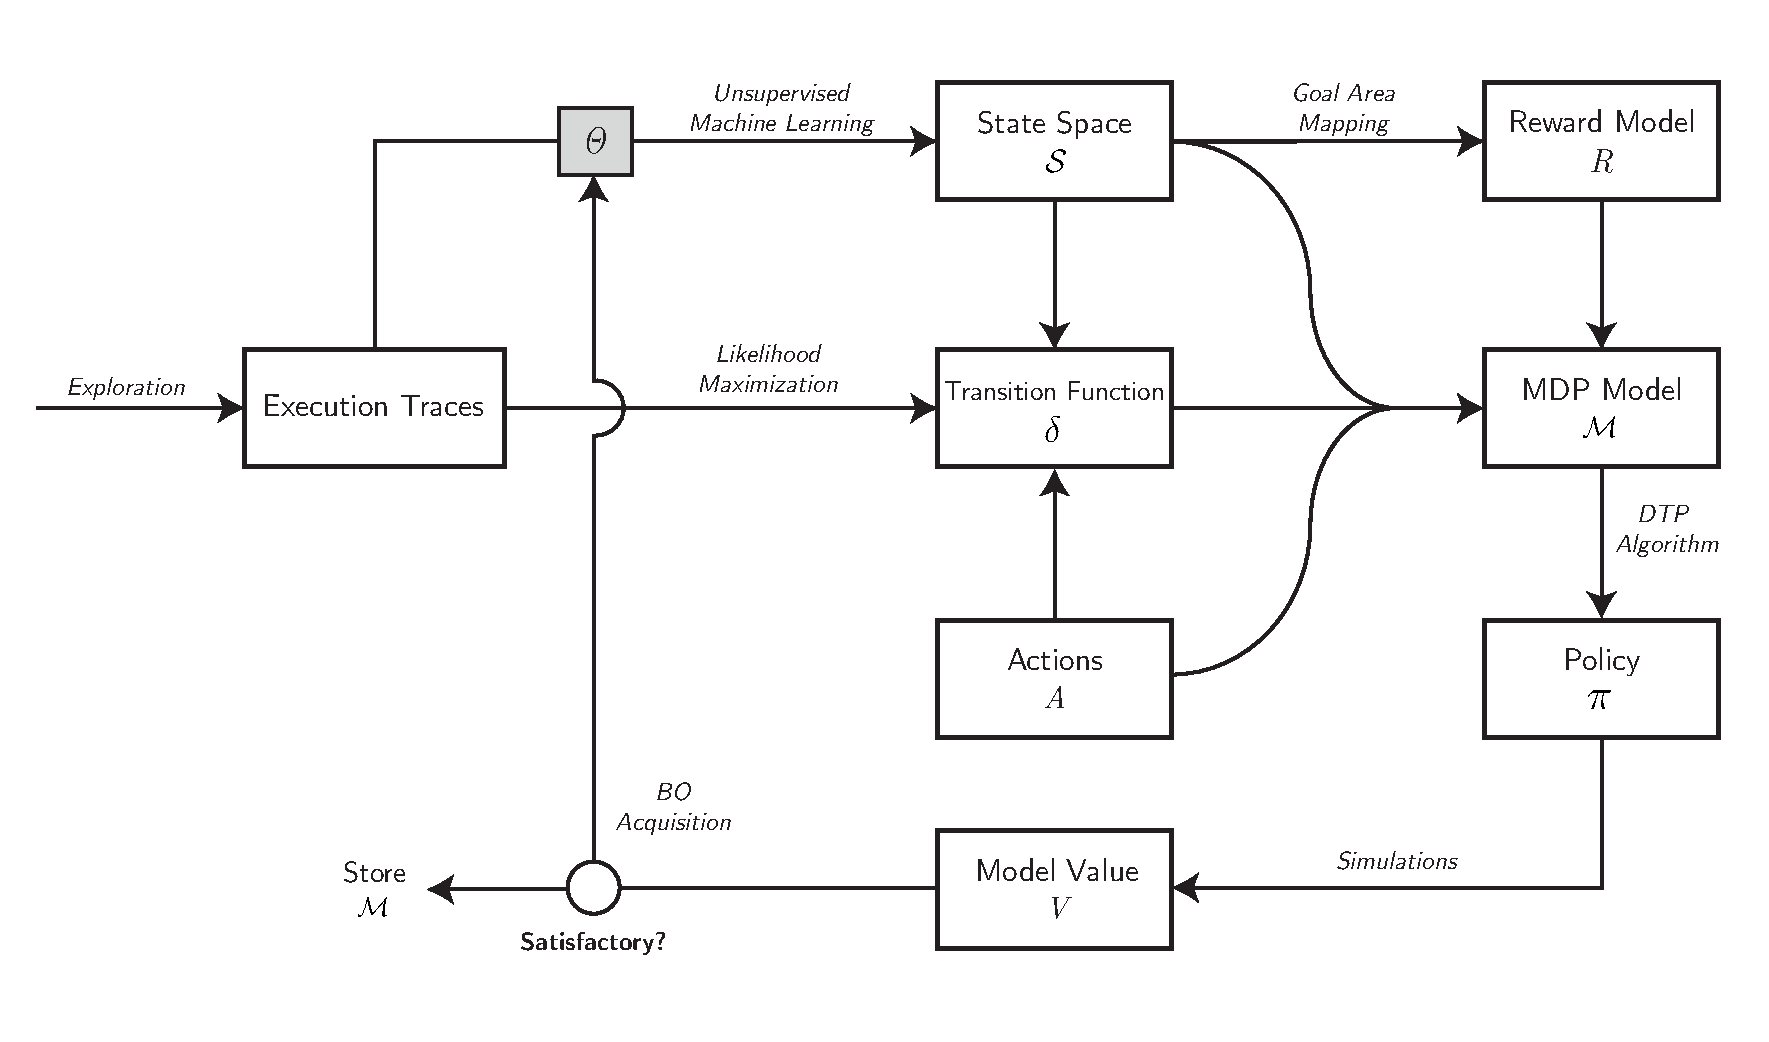
\includegraphics[width=\textwidth]{learning-cycle-complete-v2}
	\caption{Diagram of the Model Learning and Optimization Routine}
	\label{fig:learning-routine-complete}
\end{figure}

% There have been debates about the performance
% measure that should be maximized during learning {
% one point of view is that the available data should be
% used to learn all possible perceptual distinctions in the
% real world 

% One of the main issues faced in learning \acrshort{acr:mdp} models is that of deciding on the state space, while one typically does not know the size of the true state space of the real-world process that generated the training data.
%In fact this state space might even have been continuous, while the state space of the model is typically discrete.
%In particular this might form an issue in the planning phase where a reward function needs to be defined to express the goals in the \acrshort{acr:mdp}, for which there may not be a clear one-to-one mapping from real-world states to model states.

% Two approaches:
% - Clustering training data to obtain states
% - Trajectory Clustering

%\textbf{Note:} These bullet-points have not been completely updated yet although most are still relevant. Outline should be such that we first discuss the framework for model learning and optimization without considering incomplete data or doing cost-sensitive optimization, which are discussed next ('why and how').
%Probably describing the framework should be separated from the application to mobile robot navigation and how it is implemented, which should be described afterwards.
%
%\begin{itemize}
%	\item Introduction
%	\item Explain high-level algorithm idea?
%\end{itemize}
%
%\section{Application}
%\label{sec:application}
%
%% 
%
%\begin{itemize}
%	\item Mobile robot navigation
%	\item Why this application?
%	\item Generalization possible to other applications?
%\end{itemize}
%
%\section{Exploration Phase}
%\label{sec:exploration-phase}
%
%% 
%
%\begin{itemize}
%	\item Obtain a dataset of observations, for our application this concerns data about attainable positions of the robot that will be controlled
%	\item Under the assumption such a dataset is not yet available to us, this dataset is retrieved in an exploration phase
%	\item In this exploration phase, the robot should explore the environment and periodically record information about its current position while aiming to visit all the locations of importance
%	\item This exploration phase is (preferably) only carried out once
%	\item To obtain a dataset for our tests the exploration phase is carried out in a robot simulator. Should also explain what data is obtained in this exploration.
%	\item The overall algorithm is tested for multiple maps/(office-like) environments, which might differ in their dimensions, number of obstacles or `openness'.
%	\item To take into account dynamically changing environments to some extent, there are also doors that will be open or closed as time passes.
%	\item The simulations are carried out in the Morse simulator, in which the exploration is carried out by an agent that randomly navigates an environment.
%\end{itemize}
%
%\section{State Space Acquisition}
%\label{sec:state-space-aggregation}
%
%% 
%
%\begin{itemize}
%	\item Using exploration data
%	\item Unsupervised machine learning to obtain states for an MDP model (various possible methods possible: e.g., kmeans, gmm)
%	\item Unknown parameter $\delta$ of the unsupervised machine learning algorithm to be optimized
%\end{itemize}
%
%\section{Model and Policy Acquisition}
%\label{sec:model-policy-acquisition}
%
%% 
%
%\begin{itemize}
%	\item State space obtained as described in previous section
%	\item Transition function obtained based on exploration data and state space through the likelihood maximization approach.
%	\item For our application the actions are fixed and can either be \textsc{NORTH}, \textsc{EAST}, \textsc{SOUTH}, \textsc{WEST} which makes the robot navigate in the corresponding direction.
%	\item Rewards
%	\item Timesteps
%	\item Policy (various possible `solvers': value iteration, policy iteration)
%\end{itemize}
%
%\section{Bayesian Model Optimization}
%\label{sec:bayesian-model-optimization}
%
%% 
%
%\begin{itemize}
%	\item Optimization of the unknown $\delta$ parameter of the machine learning algorithm for state space aggregation
%	\item Evaluation by simulations of the found policy for the given $\delta$ parameter
%	\item ...
%\end{itemize}
%

\chapter{Experimental Setup and Results}
\label{ch:experimental-results}

%\begin{itemize}
%	\item Introduction about application and high-level explanation of what we'll be looking into
%\end{itemize}

In \autoref{ch:methodology} a framework was proposed for finding an optimal \acrshort{acr:mdp} for planning problems that involve uncertainty given a dataset describing the dynamics of the system under consideration.
The framework aims to achieve this by posing the adjustment of the parameters of model learning algorithms as an optimization task in which the yielded performance is to be maximized.
The domain of mobile robot navigation, where the problem statement is to navigate a robot between locations as fast as possible, was identified as a potentially suitable application.
This chapter discusses the experiments that were conducted to evaluate the framework for this application and the results that were obtained accordingly.
First of all, \autoref{sec:setup} elaborates upon the setup for the experiments, discussing the relevant details on the implementation of the framework for this application and the software and other resources used.
Subsequently, \autoref{sec:scenarios} discusses the different configurations that shall be used to test the framework.
This for instance involves various combinations of learning algorithms and different settings of the discount factor $\gamma$ and weight parameter $\beta$ on different environments.
In, \autoref{sec:results} the results obtained for these different configurations are presented, inspected and compared to one another, after which the most notable conclusions that can be drawn are discussed.

\section{Setup}
\label{sec:setup}

For our experiments we made an implementation of the framework in the form of a module that can be used to learn an optimal \acrshort{acr:mdp} for the navigation of a mobile robot.
This implementation allows the control of a mobile robot in simulations by an \acrshort{acr:mdp} and a corresponding policy.
The model values assessed from these simulations are used to find a globally maximizing parameter-settings of the learning algorithm used.
In this section we will describe the implementation in detail and how it is used in our experiments to find performance-maximizing \acrshortpl{acr:mdp} for a mobile robot in an office environment.

\subsection{Software}
\label{sec:software}

In this section we discuss the software that is used in the implementation of our optimization module. 
An overview of the main packages used for this implementation is presented in \autoref{tab:software-packages}.
In the remainder of this section, we briefly explain for what part of the implementation each of these packages are used, and support the choices made where necessary.

\begin{table}[pt]
\caption{Software packages used for the implementation of the model learning framework for mobile robot navigation.}
\label{tab:software-packages}\centering
\begin{tabular}{lll}
	\hline%
	\textbf{Package Name} & \textbf{Version} & \textbf{Purpose} \\
	\hline
	\texttt{bayesian-optimization} & 0.4.0 & Bayesian optimization \\
	\texttt{matplotlib} & 1.3.1 & Plotting and visualizing robot actions \\
	\texttt{numpy} & 1.12.1 & Array data storage and manipulation\\ 
	\texttt{pymdptoolbox} & 4.0\_b3 & \acrshort{acr:mdp} planning algorithms \\
	\texttt{ros-indigo-strands-desktop} & 0.0.14 & Simulation software and environments\\
	\texttt{scikit-learn} & 0.18.1 & Machine learning algorithms \\ \hline
\end{tabular}
\end{table}

\subsubsection{Python Libraries}
\label{sec:software-packages}
The module has been implemented in Python 2.7, due to its easily usable libraries for machine learning and plotting and other widely available packages, but also because of its convenient capability of interacting with the simulation software used.

For \acrshort{acr:mdp} planning, the \texttt{pymdptoolbox} library \cite{cordwellpymdptoolbox}, is used, which implements various planning algorithms for discrete-time \acrshortpl{acr:mdp}. 
To solve for optimal policies in learned \acrshortpl{acr:mdp} we rely on this library and apply the \acrshort{acr:vi} algorithm with a discount factor of $\gamma = 0.95$.
%Given the matrices with the transition probabilities and rewards and algorithm-parameters like a discount factor $\gamma$, these planning algorithms can produce a policy vector and a corresponding value function.

For the machine learning algorithms used, we employ the \texttt{scikit-learn} library. These algorithms include $k$-Means clustering and \acrfull{acr:gmm}.

For \acrlong{acr:bo} the \texttt{bayesian-optimization} library \cite{nogueirabayesianoptimization} has been employed. This library offers an implementation of the \acrshort{acr:bo} procedure based on a \acrshort{acr:gp} prior including the implementation of the most-used acquisition functions such as \acrshort{acr:mpi}, \acrshort{acr:mei} and \acrshort{acr:gp-ucb}.

The further Python packages used, have been listed in \autoref{tab:software-packages} and include \texttt{numpy} for the manipulation of arrays and matrices used in the implementation and \texttt{matplotlib} for creating the various plots shown in this chapter.

\subsubsection{Simulator and Mobile Robot}
\label{sec:simulator}

% Make figure with two subfigures
\begin{figure}[t]
\centering
\begin{minipage}{0.4\textwidth}
	\centering
	\includegraphics[width=0.3\linewidth]{scitosa5_1_model}
	\captionof{figure}{The SCITOS-A5, mobile service robot by Metralabs GmbH \cite{Metralabs}}
	\label{fig:scitosa5}
\end{minipage}
\qquad
\begin{minipage}{0.4\textwidth}
	\centering
	\vspace{23pt}
	\includegraphics[width=1.1\linewidth]{scitosa5_2_TIM}
	\vspace{-10pt}
	\captionof{figure}{The SCITOS-A5 in one of its application environments. Shown here is robot \textit{TIM}, used for leading visitors of the German Technical Museum in Berlin through the exhibits \cite{Metralabs}.}
	\label{fig:scitosa5_2}
\end{minipage}
\end{figure}

For performing simulations the \textit{MORSE} simulator \cite{morse_simpar_2012}, a generic simulator for academic robots, has been used in combination with the \textit{ROS} middleware to control the robot in the environment.
The simulations are performed with the Metralabs GmbH \textit{SCITOS-A5} \cite{Metralabs}, depicted in \autoref{fig:scitosa5}, an industry-standard mobile service robot designed specifically for interacting with humans and guiding them to products or exhibits (e.g., see \autoref{fig:scitosa5_2}).
This robot is equipped with several sensors which can be used for navigation and \acrfull{acr:hri}, such as an omni-directional camera, 24 ultrasonic sensors, a collision sensor and a SICK laser range finder \cite{gross2008shopbot}.
As described in \autoref{sec:implementation} we are particularly interested in the odometric capabilities of the robot for the implementation that has been used in our experiments.
The \texttt{strands-desktop} meta-package (developed as part of the \textit{STRANDS} project \cite{hawes2016strands}) was used to obtain all required simulation software mentioned above with ease, in which the environments used in the simulations of our experiments are contained as well.



%
%\vspace{12pt}
%\noindent\fbox{\textbf{TODO:} Not completely finished yet.}

%Software used for the implementation:
%\begin{itemize}
%	\item Programming Language: \textit{Python (2.7)} together with \texttt{scikit-learn}, \texttt{pymdptoolbox}, \texttt{bayesian-optimization} packages + explain what each of them are used for
%	\item Simulator: \textit{Morse}
%	\item Scitos-A5 robot, mobile service robot (plus \textit{short} discussion of what this robot has been used for in the real world)
%	\item Control movements of robot in simulator through \textit{ROS}
%\end{itemize}

\subsection{Datasets}
\label{sec:datasets}

\begin{table}[pt]
	\caption{Metadata about the execution traces obtained}
	\label{tab:datasets-environments}\centering
	\begin{tabular}{|l|l|l|}
	\hline
	\textbf{Environment} & \textbf{Area} & \textbf{Number of entries in dataset} \\
	\hline
	\texttt{tum\_kitchen}&               &                                       \\
	\hline
	\texttt{uol\_bl}&               &            						\\ \hline          
	\end{tabular}
\end{table}

In order to be able to learn \acrshortpl{acr:mdp} from data and establish the optimization, we should obtain a dataset that  describes the environment the robot will operate in.
This dataset should describe possible robot poses and to what other poses the execution of the possible actions may lead to, in order to properly describe the dynamics of the system.

For our implementation and the experiments that have been carried out, execution traces have been obtained by letting the robot follow a random action policy during which subsequent poses and actions are logged to a file.
This exploration is performed inside the simulator both for a relatively small environment (i.e., \texttt{tum\_kitchen}) and  large environment (i.e., \texttt{uol\_bl}) obtained from a repository of the \textit{STRANDS} project.

%Explain how the data-sets are obtained. 
%- For multiple environments - What is obtained. - How the data is obtained.

\subsection{Implementation}
\label{sec:implementation}

Details on the implementation; how the framework/routine is implemented for this application. Discuss how the following aspects are taken care of in the implementation:
\begin{itemize}
	\item Environments
	\item Exploration / Data Gathering
	\item Optimization
	\item Simulations of following policy
\end{itemize}

\subsubsection{title}

\section{Scenarios}
\label{sec:scenarios}

%Discuss the different configurations that are to be compared
%\begin{itemize}
%	\item Fixed values for $\beta$-parameter vs. gradually decreasing from $1$ to $0$
%	\item Multiple environments: small (\texttt{tum\_kitchen}); large (\texttt{uol\_bl})
%	\item Model-learning algorithms: direct clustering vs. trajectory clustering; $k$-means vs. GMM
%	\item Data-sets of different sizes
%\end{itemize}

\noindent Configurations for the basic optimization framework (only based on simulations):
\begin{itemize}
	\item Fixed value for $\beta$ (i.e., which weighs $V_\mathit{DTP}$): $0$, $0.25$ and $0.5$
	\item Acquisition functions: \acrshort{acr:gp-ucb}, \acrshort{acr:mei}
	\item GMM vs. $k$-Means (vs. trajectory clustering if time available)
	\item All available data, 75\% and 50\%
	\item Discount factor: $\gamma = 0.95$
	\item Small environment: \texttt{tum\_kitchen}; and large environment: \texttt{uol\_bl}
\end{itemize}
We need to record: number of iterations, total time passed, optimum found ($\theta_\textnormal{max}$ and $V_{\mathcal{M},\textnormal{max}}$)

\vspace{12pt}
\noindent For the cost-incremental extension we could try to observe what happens when we decrease $\beta$ gradually over time.

\vspace{12pt}
\noindent Do we want to do something with `variable resolution' as post-processing step in the experiments?

\vspace{12pt}
\noindent\fbox{\textbf{TODO:} Table to be added describing the configurations/scenarios for the experiments.}

\section{Results}
\label{sec:results}

\begin{itemize}
	\item First show results of optimization only based on simulation outcomes
	\item Then show results for the cost-incremental extension of the framework
\end{itemize}


\chapter{Conclusion}
\label{ch:conclusions}



%% Use letters for the chapter numbers of the appendices.
\appendix

%\input{appendix-a}

% Acronyms and Glossary
\printglossary[type=\acronymtype]
\addcontentsline{toc}{chapter}{Acronyms} % toc gives different font
%\printglossary

\bibliography{references}

\end{document}

% Using the order described here: http://academia.stackexchange.com/questions/5569/where-in-a-thesis-should-a-glossary-be-positioned

%TODO Check for consistent spelling, probably update glossary and check for use of dashes and change words to reach consistency

%TODO List of Figures?